\documentclass[twoside,11pt]{article}

% Any additional packages needed should be included after jmlr2e.
% Note that jmlr2e.sty includes epsfig, amssymb, natbib and graphicx,
% and defines many common macros, such as 'proof' and 'example'.
%
% It also sets the bibliographystyle to plainnat; for more information on
% natbib citation styles, see the natbib documentation, a copy of which
% is archived at http://www.jmlr.org/format/natbib.pdf

\usepackage{jmlr2e}
\usepackage{comment}
\usepackage{graphicx}
\graphicspath{ {./images/} }

% Definitions of handy macros can go here

\newcommand{\dataset}{{\cal D}}
\newcommand{\fracpartial}[2]{\frac{\partial #1}{\partial  #2}}



% Heading arguments are {volume}{year}{pages}{submitted}{published}{author-full-names}

% \jmlrheading{1}{2000}{1-48}{4/00}{10/00}{author-full-names}

% Short headings should be running head and authors last names


\ShortHeadings{InterpretML - Draft}{Meil\u{a}, Meil\u{a}, Meil\u{a} and Jordan}
\firstpageno{1}

\begin{document}

\title{InterpretML: A Unified Framework for Machine Learning Interpretability}

\author{\name Harsha Nori \email hanori@microsoft.com \\
        \name Samuel Jenkins \email sajenkin@microsoft.com \\
        \name Paul Koch \email paulkoch@microsoft.com \\
       \name Rich Caruana \email rcaruana@microsoft.com \\
       \addr Microsoft Corporation\\
       1 Microsoft Way\\
       Redmond, WA 98052, USA}

% \editor{Leslie Pack Kaelbling}

\maketitle

\begin{abstract}%   <- trailing '%' for backward compatibility of .sty file

InterpretML is an open-source Python package which exposes machine learning interpretability algorithms to practitioners and researchers. InterpretML exposes two types of interpretability -- ''glassbox'', which are machine learning models designed for interpretability (ex: Linear models, Rule Lists), and ''blackbox'' explainability techniques for explaining existing systems (ex: Partial Dependence, LIME). The package enables practioners to easily compare multiple interpretability algorithms by exposing all methods under a unified API, and by having a built-in, extensbile visualization platform. InterpretML also includes the first implementation of the Explainable Boosting Machine, a powerful, interpretable model that can be as accurate as many blackbox models. Source code can be downloaded from \href{https://github.com/microsoft/interpret}{github.com/microsoft/interpret}. 

\end{abstract}

\begin{keywords}
Interpretability, Explainable Gradient Boosting, Glassbox, Blackbox
\end{keywords}

\section{Introduction}

Machine learning interpretability has become an increasingly important tool for scientists to debug their models, meet growing regulatory requirements, and allow AI systems to work better with humans. InterpretML exposes many state-of-the-art interpretability techniques -- both ''glassbox'' models, which are inherently explainable ML models, and ''blackbox'' interpretability techniques, which can generate explanations for any ML pipeline -- under a unified API. This enables scientists to compare and contrast multiple interpretability methods, and pick the best one for their needs. 


% {\noindent \em Remainder omitted in this sample. See http://www.jmlr.org/papers/ for full paper.}

% Acknowledgements should go at the end, before appendices and references

\section{Package Design}

PICTURE: Algorithm comparison checklist. 

\subsection{Uniform API}

All techniques inherit from a base class, register what type of explanation (local, global, etc.). 

Glassbox models follow an extended version of the sci-kit learn specification. Initialize, fit, predict. Modifications include extensions to allow feature names to be passed. 

Blackbox models follow an API that allows each method to ''take what they want''. Predictfn, data, feature names, names. 

\subsection{Visualization}

Every explanation supports a built in visualization. Can extract raw data with data method. Supported types include plain text (markdown), plotly graphs, dash components. Everything also works in a dashboard designed to make it easy to compare algorithms. 

\section{Explainable Boosting Machine}

Historically, the most intelligible models were not very accurate, and the most accurate models were not intelligible. Microsoft Research has developed an algorithm called the Explainable Boosting Machine (EBM)* which has both high accuracy and intelligibility. EBM uses modern machine learning techniques like bagging and boosting to breathe new life into traditional GAMs (Generalized Additive Models). This makes them as accurate as random forests and gradient boosted trees, and also enhances their intelligibility and editability.
\vskip 0.1in
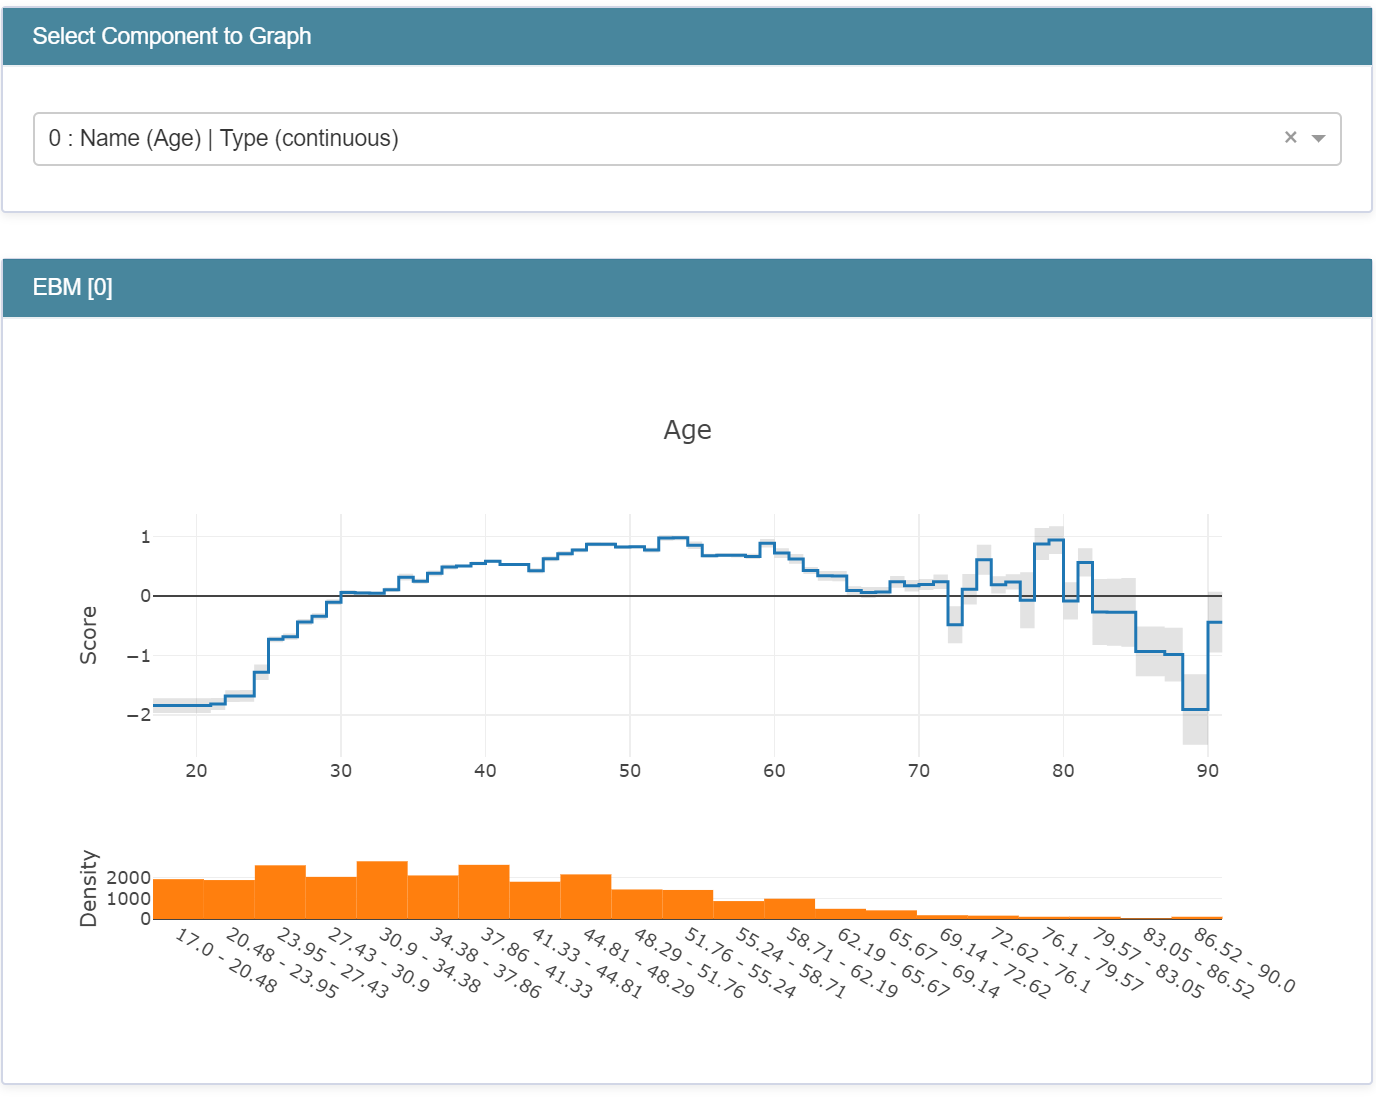
\includegraphics[scale=0.24]{images/ebm_global_age.PNG}
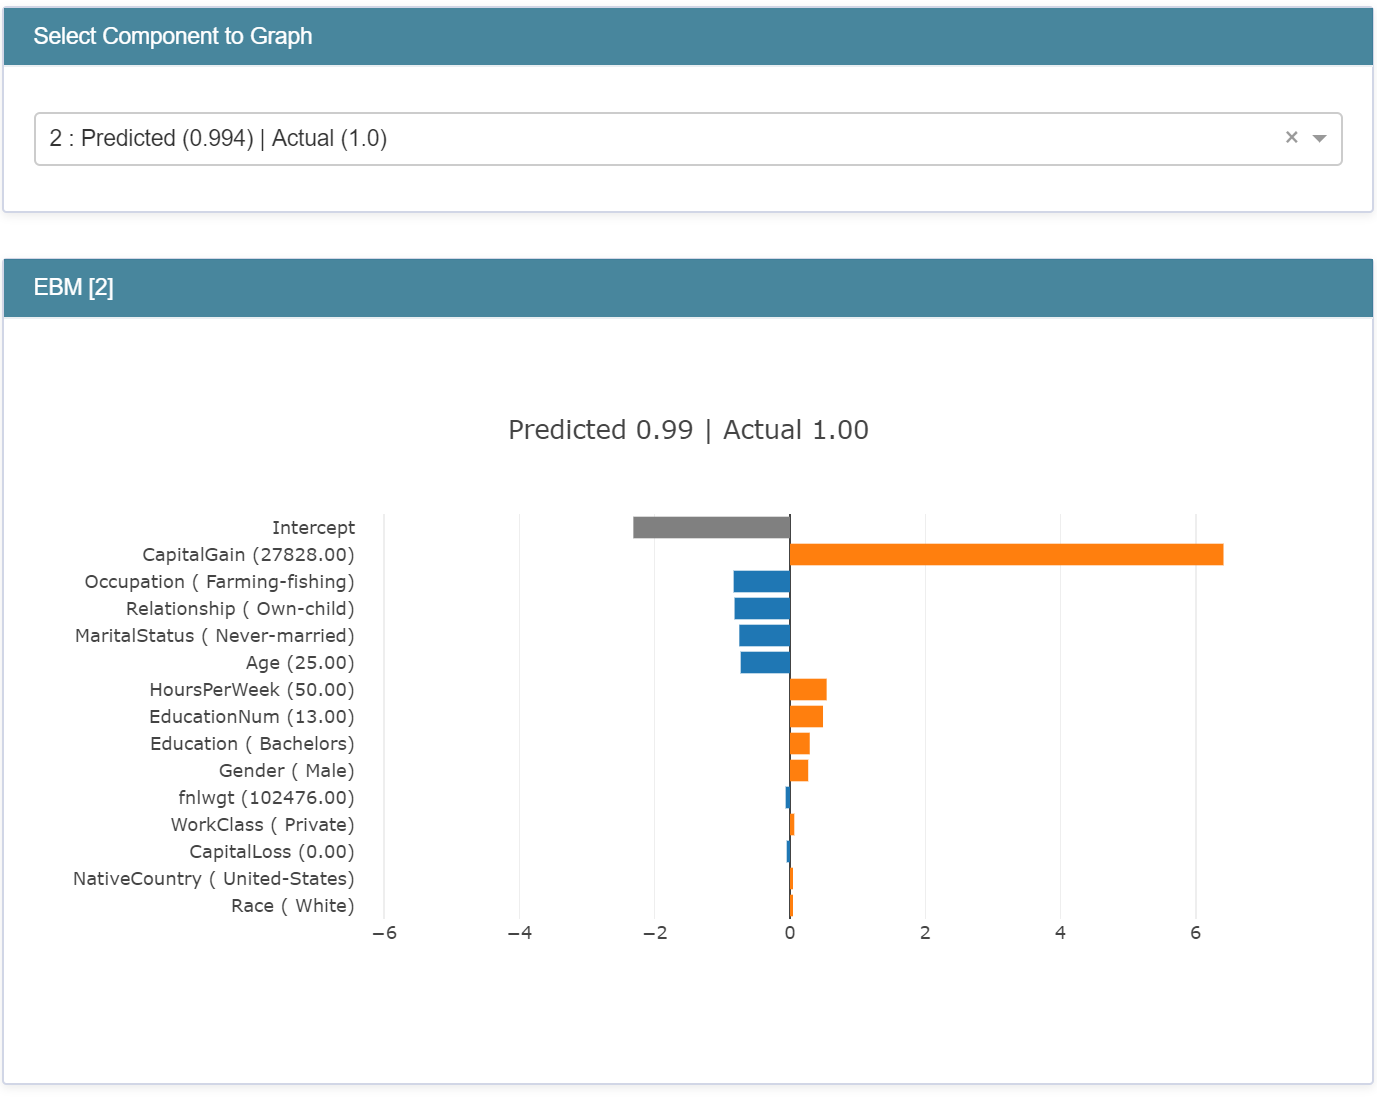
\includegraphics[scale=0.24]{images/ebm_local.PNG}

EBM provides explanations at both a global and local level. 

\subsection{Comparisons}

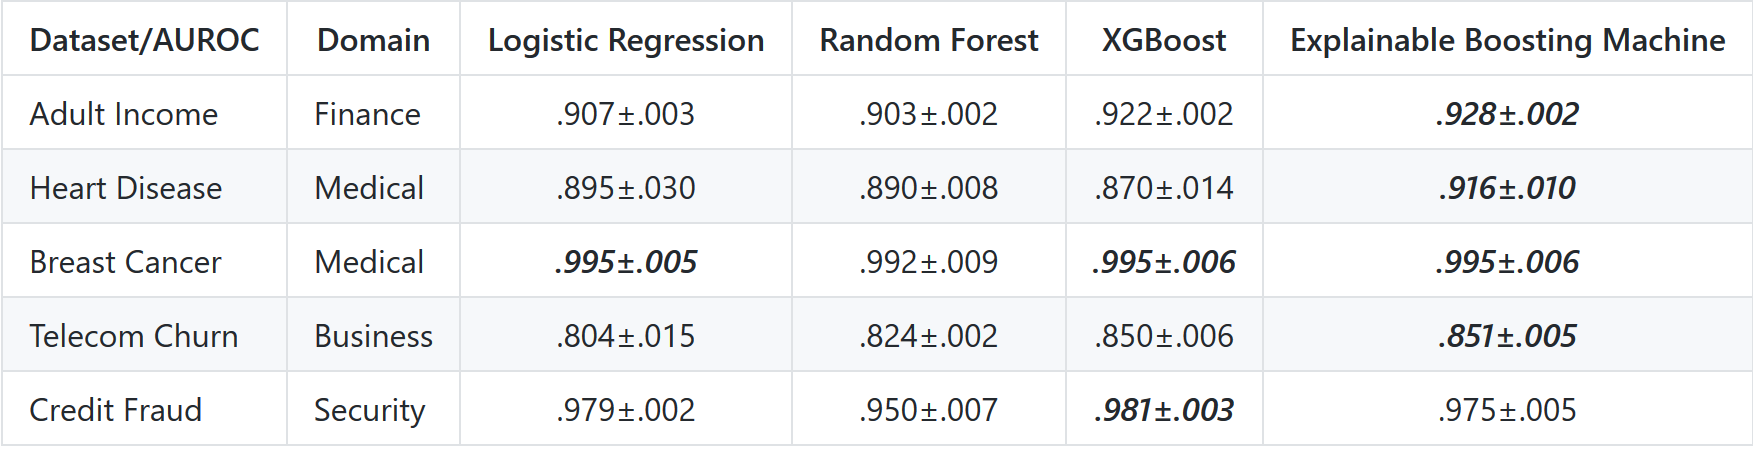
\includegraphics[scale=0.65]{performance_comparison.PNG}

EBM tends to perform quite well compared to state of the art methods like XGBoost and Random Forest, while providing perfect interpretability. 

PICTURE: Accuracy (Classification vs other standard algorithms). 
PICTURE: Speed (train and predict time)

\section{Discussion}
Discuss this.

\acks{We would like to acknowledge everyone on our \href{https://github.com/microsoft/interpret/blob/master/ACKNOWLEDGEMENTS.md}{acknowledgements.md} file for their support on project. }

% Manual newpage inserted to improve layout of sample file - not
% needed in general before appendices/bibliography.

\newpage

\begin{comment}

\appendix
\section*{Appendix A.}
\label{app:theorem}

% Note: in this sample, the section number is hard-coded in. Following
% proper LaTeX conventions, it should properly be coded as a reference:

%In this appendix we prove the following theorem from
%Section~\ref{sec:textree-generalization}:

In this appendix we prove the following theorem from
Section~6.2:

\noindent
{\bf Theorem} {\it Let $u,v,w$ be discrete variables such that $v, w$ do
not co-occur with $u$ (i.e., $u\neq0\;\Rightarrow \;v=w=0$ in a given
dataset $\dataset$). Let $N_{v0},N_{w0}$ be the number of data points for
which $v=0, w=0$ respectively, and let $I_{uv},I_{uw}$ be the
respective empirical mutual information values based on the sample
$\dataset$. Then
\[
	N_{v0} \;>\; N_{w0}\;\;\Rightarrow\;\;I_{uv} \;\leq\;I_{uw}
\]
with equality only if $u$ is identically 0.} \hfill\BlackBox

\noindent
{\bf Proof}. We use the notation:
\[
P_v(i) \;=\;\frac{N_v^i}{N},\;\;\;i \neq 0;\;\;\;
P_{v0}\;\equiv\;P_v(0)\; = \;1 - \sum_{i\neq 0}P_v(i).
\]
These values represent the (empirical) probabilities of $v$
taking value $i\neq 0$ and 0 respectively.  Entropies will be denoted
by $H$. We aim to show that $\fracpartial{I_{uv}}{P_{v0}} < 0$....\\

{\noindent \em Remainder omitted in this sample. See http://www.jmlr.org/papers/ for full paper.}



\vskip 0.2in


\end{comment}

\nocite{*}
\bibliography{sample}

\end{document}